\documentclass[xcolor=dvipsnames]{beamer}

\usepackage{xcolor}
\usepackage[ngerman]{babel} % deutsche Silbentrennung
\usepackage[utf8]{inputenc} % wegen deutschen Umlauten
\usepackage{pdfpages}
\usepackage{graphicx}
\usepackage{pst-node}% http://ctan.org/pkg/pst-node
\usepackage{eurosym}


\usetheme{metropolis}           % Use metropolis theme
\title{The smallest grammar problem}
\date{05. Juli 2019}
\author{Edgar Dorausch}
%\institute{Centre for Modern Beamer Themes}
\begin{document}
\maketitle

\newcommand{\Gap}{$ $ \linebreak}
\newcommand{\FrameName}{
	\ifthenelse{\equal{\subsecname}{}}{
		\secname
	}{
		\secname \thinspace -\thinspace\subsecname
	}
}

\newcommand{\Fresh}{\ddagger}
\newcommand{\Hint}[1]{\textcolor{gray}{#1}}


\section{Motivation und Anwendung}

\begin{frame}{\FrameName}
	\begin{itemize}[<+->]
		\item Mustererkennung
		\item Kompression
	\end{itemize}
\end{frame}

\section{Definitionen und Wiederholung}
\begin{frame}{\FrameName}
	\begin{block}{Kontextfreie Grammatik}
		\Gap
		Eine KFG ist ein Quadrupel $(\Sigma,\Gamma,S,\Delta)$ mit
		\begin{itemize}
			%	\item \alert<4>{This is\only<4>{ really} important}
			\item $\Sigma$ - Terminalalphabet
			\item $\Gamma$ - Nichtterminalalphabet
			\item $S$ - Startsymbol
			\item $\Delta$ - Menge von Regeln der Form $T\rightarrow\alpha$\linebreak
			$T \in \Gamma$;
			$\alpha \in (\Sigma \cup \Gamma)^\ast$
		\end{itemize}
	\end{block}
	
\end{frame}

\begin{frame}{\FrameName}
\begin{alert}{Besonderheit!:}
	\Gap
	Die Grammatiken sollen nur ein Wort erzeugen. Deshalb:
	\begin{itemize}
		
		\item Grammatik muss azyklisch sein
		\item Für jedes $T \in \Gamma$ existiert nur eine Regel in $\Delta$
	\end{itemize}
\end{alert}
\end{frame}

\begin{frame}{\FrameName}
\begin{block}{Expansion  eines Strings $\alpha$}
	\Gap
	Erhält man durch erschöpfendes Anwenden der Regeln in einer Grammatik bis nur noch Terminale enthalten sind. \linebreak
	Notation: $\langle \alpha \rangle$
\end{block}
\end{frame}

\begin{frame}{\FrameName}
\begin{block}{Expansionslänge}
	\Gap
	Anzahl der Zeichen in der Expansion eines Strings $\alpha$ \linebreak
	Notation: $[\alpha]  = \lvert \langle \alpha \rangle \lvert$
\end{block}
\end{frame}

\begin{frame}{\FrameName}
\begin{block}{Größe einer Grammatik G}
	\Gap
	Anzahl der Zeichen in den rechten Seiten der Grammatikregeln\linebreak
	Notation: $m = \lvert G \lvert = \sum\limits_{(T \rightarrow \alpha) \in \Delta} \langle \alpha \rangle$ \linebreak $ $\linebreak
	Größe der kleinsten Grammatik für einen String: $m^*$
\end{block}
\end{frame}

\begin{frame}{\FrameName}
\begin{block}{Beispiel}
	$$
	G \colon \begin{Bmatrix} 
		S \rightarrow rhaTber \textvisiblespace TTa \\
		T \rightarrow bar
	\end{Bmatrix}
	$$
	
	$\langle S \rangle = rhabarber \textvisiblespace barbara$ \linebreak
	$[S] = 17$ \linebreak
	$\lvert G \lvert = 11$
\end{block}
\end{frame}

\begin{frame}{\FrameName}
\begin{block}{Approximation Ratio}
	\Gap
	Sei $G_A$ die Grammatik, die von einem Algorithmus $A$ erzeugt wird.
	$$
	a(n) = \alert<2>{\max\limits_{\alpha \in \Sigma^n}}\frac{
		\textrm{$\lvert G_A \lvert$ für $\alpha$}
	}{
		\textrm{$m^*$ für $\alpha$}
	}
	$$
	\begin{center}\alert{
			
			\only<2>{Worstcase!}
		}
	\end{center}
	
\end{block}
\end{frame}

\begin{frame}{\FrameName}
\begin{table}
	\caption{Landau Notation}
	\begin{tabular}{ r p{3.5cm} l}
		
		$f \in o(g)$ & "$f < g$" \\
		%$\only<1>{f \in \mathcal{O}(g)}\only<2>{\alert{f \in \mathcal{O}(g)}}$ & "$f\leq g$" \\
		\textcolor{gray}{(Upper bound)} $f \in \mathcal{O}(g)$ & "$f\leq g$" \\
		$f \in \Theta(g)$ & "$f = g$"\\
		\textcolor{gray}{(Lower bound)} $f \in \Omega(g)$ & "$f \geq g$"\\
		$f \in \omega(g)$ & "$f > g$"\\
	\end{tabular}
\end{table}
\end{frame}

\section{Komplexität}
	
\begin{frame}{\FrameName}
\begin{itemize}[<+->]
	\item Vertex Cover lässt sich auf SGP reduzieren
	\item Zusammenhang mit Addition Chains \textcolor{gray}{(nicht im Vortrag)}
\end{itemize}
\end{frame}

\begin{frame}{\FrameName}
\begin{block}{Vertex Cover}
	\Gap
	Suche (minimale) Menge von Knoten, sodass jede Kante mindestens einen dieser Knoten enthält.\linebreak
	$ $\linebreak
	
	\only<1>{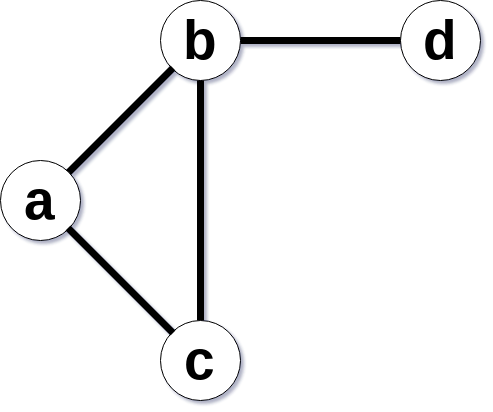
\includegraphics[width=0.25\textwidth]{Images/VertexCover/blank}}
	\only<2>{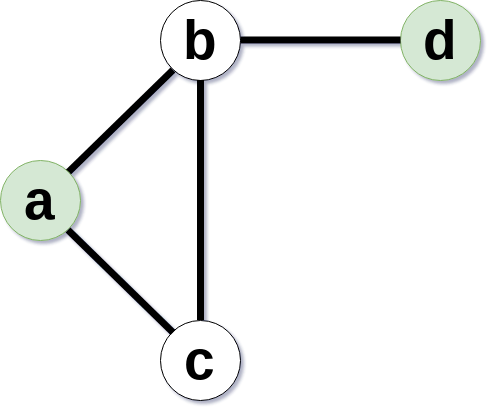
\includegraphics[width=0.25\textwidth]{Images/VertexCover/wrong}}
	\only<3>{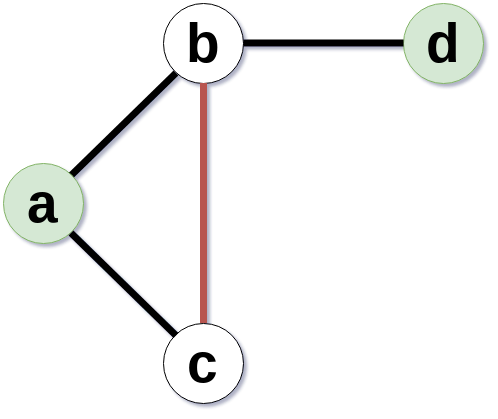
\includegraphics[width=0.25\textwidth]{Images/VertexCover/wrongMarked} \alert{(Kein Vertex Cover!)}}
	\only<4>{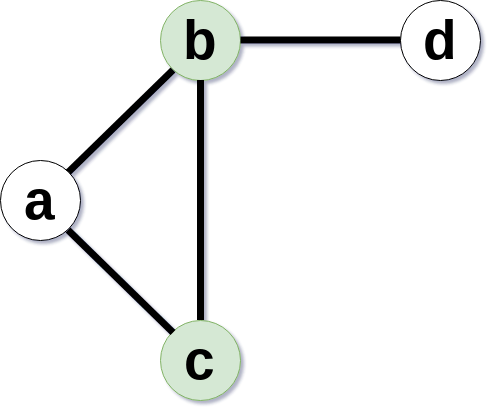
\includegraphics[width=0.25\textwidth]{Images/VertexCover/right}}
\end{block}
\end{frame}

\newcommand{\ExampleGraphV}{V = \{a,b,c,d\}}
\newcommand{\ExampleGraphE}{E = 
	\begin{Bmatrix}
		\{a,b\},
		\{a,c\},
		\{b,c\},
		\{b,d\}
	\end{Bmatrix}
}

\begin{frame}{\FrameName}
\begin{block}{NP-härte}
	\begin{itemize}[<+->]
			\item Betrachte nur Graphen mit maximalen Knoten-Grad 3
			\item Überführung von Graphen zu Wörtern
			\item Zeige, dass man über die kleinsete Grammatik einen Vertex Cover bestimmen kann
			\item Berechne Upper Bound für effiziente Approximation \linebreak (außer $P=NP$)
		\end{itemize}
\end{block}
\end{frame}

\begin{frame}{\FrameName}
\begin{block}{Beispiel Graph}
	\Gap
	$$\ExampleGraphV$$ 
	$$\ExampleGraphE$$
	\begin{center}
		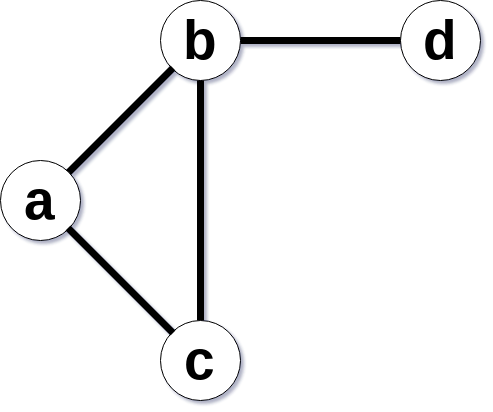
\includegraphics[width=0.35\textwidth]{Images/VertexCover/blank}
	\end{center}
\end{block}
\end{frame}

\newcommand{\ProdRuleOne}[1]{(\# #1 \Fresh #1\#  \Fresh )^2}
\newcommand{\ProdRuleTwo}[1]{\# #1 \#  \Fresh}
\newcommand{\ProdRuleThree}[2]{\# #1 \# #2\#  \Fresh}
\newcommand{\PhantomAlpha}{\phantom{\alpha_{Beispiel} = (}}
\newcommand{\ReductionExample}{
	$
		\alpha_{Beispiel} =
		\textcolor{OrangeRed}{
			\foreach \n in {a,b,c,d}{\ProdRuleOne{\n}}
		} \linebreak
		\PhantomAlpha
		\textcolor{PineGreen}{
			\foreach \n in {a,b,c,d}{\ProdRuleTwo{\n}}
		} \linebreak
		\PhantomAlpha
		\textcolor{RoyalBlue}{
			\ProdRuleThree{a}{b}
			\ProdRuleThree{a}{c}
			\ProdRuleThree{b}{c}
			\ProdRuleThree{b}{d}
		} \linebreak
	$
}

\begin{frame}{\FrameName}
\begin{block}{Graphen zu String überführen}
	\Gap
	$
	\alpha =
	\textcolor{OrangeRed}{
		\prod\limits_{v_i \in V}\ProdRuleOne{v_i}}
	\textcolor{PineGreen}{
		\prod\limits_{v_i \in V}(\ProdRuleTwo{v_i})}
	\textcolor{RoyalBlue}{
			\prod\limits_{\{v_i,v_j\} \in E}(\ProdRuleThree{v_i}{v_j})}
	$

	
	\only<2>{
		\Gap
			$\ExampleGraphV; \ExampleGraphE$ \newline
		\Gap
		\ReductionExample
	}
\end{block}
\end{frame}

\begin{frame}{\FrameName}
	\ReductionExample
\begin{block}{Eigenschaften der kleinsten Grammatik}
	\begin{itemize}[<+->]
		\item Jedes Nichtterminal expandiert zu $\#v_i$, $v_i\#$ oder $\#v_i\#$
		\item Enthält Regeln der Form $T_j \rightarrow \#v_i$ und $T_j \rightarrow v_i\#$
		\item $C = \{v_i \in V | \exists T_j \rightarrow \#v_i\#\}$ ist (minimale) Vertex Cover
	\end{itemize}
\end{block}
\end{frame}

\begin{frame}{\FrameName}
\begin{block}{Approximation Ratio}
	\begin{itemize}[<+->]
		\item $m^* = 15|V| + 3|E| + |C|$
		\item Es ist ($NP$) hart Vertex Cover kleiner als $\frac{145}{144} \cdot |C|$ zu finden ($\frac{145}{144}\approx 1,006944...$)
		\item $\rho = \frac{15|V| + 3|E| + \frac{145}{144}|C|}{15|V| + 3|E| + |C|}$
		\item $\rho \geq \frac{15|V| + 3 \cdot \frac{3}{2}|V| + \frac{145}{144}(\frac{1}{3}|V|)}{15|V| + 3 \cdot \frac{3}{2}|V| + \frac{1}{3}|V|} = \frac{8569}{8568} \approx 1,0001167...$
	\end{itemize}
\end{block}
\end{frame}

\section{Algorithmen}

\subsection{Vorüberlegungen}

\newcommand{\LowerBound}{\textcolor{TealBlue}{f_l(n)}}
\newcommand{\UpperBound}{\textcolor{Salmon}{f_u(n)}}

\begin{frame}{\FrameName}
\begin{block}{Lower bound bestimmen}
	\begin{itemize}[<+->]
		\item Definiere $\alpha$ \textcolor{gray}{(n = $|\alpha |$)}
		\item Bestimme lower bound von $m$ \linebreak \textcolor{gray}{$m \in \Omega(\LowerBound)$}
		\item Bestimme upper bound von $m^*$ \linebreak \textcolor{gray}{$m^* \in \mathcal{O}(\UpperBound)$}
	\end{itemize}
	\only<4>{
		$\Rightarrow$
		\fbox{
		$a(n) \in \Omega(\frac{
			\LowerBound
		}{
			\UpperBound
		})$
		}}
\end{block}
\end{frame}

\subsection{LZ78}

\begin{frame}{\FrameName}
\begin{block}{LZ78 - Datenstrukturen}
	\begin{itemize}[<+->]
		\item Strings werden als Sequenzen von Paaren $(i,c)$ dargestellt \linebreak \Hint{$i$...Index eines Vorgänger-Paares oder $0$$; c \in \Sigma$}
		\item Jedes Paar repräsentiert einen Substring
		\item Wenn $i$ gleich $0$ dann ist dieser Substring gleich $c$
		\item Andernfalls ist der Substring des $i$-ten Parres gefolgt von $c$
	\end{itemize}
\end{block}
\end{frame}

\begin{frame}{\FrameName}
\begin{block}{Beispiel}
	\Gap
	\Gap
	\only<1>{
		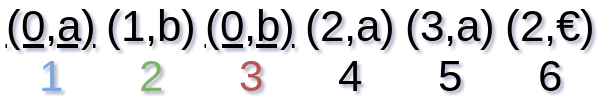
\includegraphics[width=\textwidth]{Images/LZ78/blank}}
	\only<2>{
		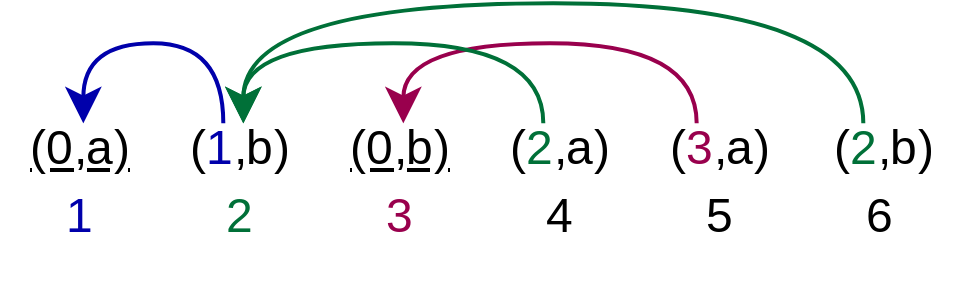
\includegraphics[width=\textwidth]{Images/LZ78/withRef}}
	\only<3>{
		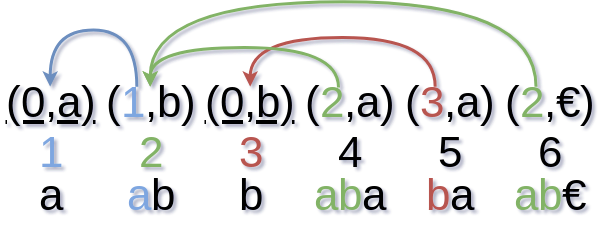
\includegraphics[width=\textwidth]{Images/LZ78/full}}
\end{block}
\end{frame}

\begin{frame}{\FrameName}
\begin{block}{LZ78 - Algorithmus}
	\begin{itemize}[<+->]
		\item String wird Schrittweise in einem Durchlauf von links nach rechts in eine Sequenz von Paaren übersetzt
		\item Finde in jedem Schritt das kürzeste Präfix $\gamma$ des verbleibenden Strings das nicht Expansion eines bereits erzeugten Paars ist
		\item Am Ende des Strings muss eventuell ein weiteres Zeichen hinzugefügt werden
		\item Ein neues Paar wird an die Liste angehangen:
		\begin{enumerate}
			\item<4-> Wenn da $\gamma = 1$ ist füge $(0,\gamma)$ hinzu
			\item<5-> Andernfalls ist $\gamma = \alpha c$. \linebreak $\alpha$ ... Expansion eines Paars mit dem Index $i_\alpha$ \linebreak $\Rightarrow$ Paar: $(i,c)$
		\end{enumerate}
	\end{itemize}
\end{block}
\end{frame}

% Marking string sequence
\newcommand{\M}[1]{\textcolor{OrangeRed}{#1}}

\begin{frame}{\FrameName}
\begin{block}{Beispiel}
	\begin{description}[<+->]
		\item \M{a}abbababaab\euro
		\item (0,a) \M{ab}bababaab\euro
		\item (0,a) (1,b) \M{b}ababaab\euro
		\item (0,a) (1,b) (0,b) \M{aba}baab\euro
		\item (0,a) (1,b) (0,b) (2,a) \M{ba}ab\euro
		\item (0,a) (1,b) (0,b) (2,a) (3,a) \M{ab\euro}
		\item (0,a) (1,b) (0,b) (2,a) (3,a) (2,\euro)
	\end{description}
\end{block}
\end{frame}

\begin{frame}{\FrameName}
\begin{block}{LowerBound}
	\begin{center}
		\fbox{$ \alpha_k = a^{k(k+1)/2}(ba^k)^{(k+1)^2} $}
	\end{center}
	\begin{itemize}[<+->]
		\item $|\alpha_k | = k \frac{k+1}{2} + (1+k)(k+1)^2$ \linebreak
			$\phantom{|\alpha_k |} = k^3 + \frac{7}{2}k^2 + \frac{7}{2}k + 1$
		\item $ n = |\alpha_k | \in \Theta(k^3)$
	\end{itemize}
\end{block}
\end{frame}

\begin{frame}{\FrameName}
\begin{block}{UpperBound $m^*$}
	\begin{center}
		\fbox{$ \alpha_k = a^{k(k+1)/2}(ba^k)^{(k+1)^2} $}
	\end{center}
	\begin{itemize}[<+->]
		\item $m^* \in \mathcal{O}(1+ log(\frac{k^2+k}{2}) + log(k+1)^2 + 1+ log(k))$
		\item $m^* \in \mathcal{O}(log \thinspace k)$
		\item $m^* \in \mathcal{O}(log \thinspace n^\frac{1}{3}) = \mathcal{O}(log \thinspace n)$
	\end{itemize}
\end{block}
\end{frame}

\begin{frame}{\FrameName}
\begin{block}{LowerBound m}
	\begin{center}
		\fbox{$ \alpha_k = a^{k(k+1)/2}(ba^k)^{(k+1)^2} $}
	\end{center}
	\begin{itemize}[<+->]
		\item String wird in zwei Phasen in eine Paar-Sequenz übersetzt
		\item Erste Phase: alle Strings $a...a^k$ zu Paaren übersetzt
		\item Zweite Phase: $a^iba^j$ für alle $i,j \in [0,k]$ wird ein Paar erstellt
		\item $m \in \Omega(\sum_{z=1}^k z + (k+1)^2) = \Omega(k^2)$
		\item $m \in \Omega(n^{2/3})$
	\end{itemize}
\end{block}
\end{frame}

\begin{frame}{\FrameName}
\begin{block}{LowerBound}
	\begin{center}
		\fbox{$ \alpha_k = a^{k(k+1)/2}(ba^k)^{(k+1)^2} $}
	\end{center}
	\begin{itemize}[<+->]
		\item $m^* \in \mathcal{O}(log \thinspace n)$
		\item $m \in \Omega(n^{2/3})$
		\item $a(n) \in \Omega(\frac{n^{2/3}}{log \thinspace n})$
	\end{itemize}
\end{block}
\end{frame}

\subsection{global algorithms}
\begin{frame}{\FrameName}
	\begin{block}{TODO}
	\Gap
	$a^2 + b^2 = c^2$
\end{block}
\end{frame}

\subsection{LZ77 variant}
\begin{frame}{\FrameName}
	\begin{block}{TODO}
	\Gap
	Basiert anscheinend auf $BB[\alpha]-Trees$
\end{block}
\end{frame}

\end{document}